\pdfobjcompresslevel=0
\pdfcompresslevel=0

\documentclass[a5paper, DIV=14, headings=openany, twoside=true,fontsize=10pt, titlepage]{scrreprt}
\usepackage[T1,T2A]{fontenc}
\usepackage[utf8]{inputenc}
\usepackage[english, russian]{babel} 
\usepackage{indentfirst}
\usepackage{subfig}
\usepackage{graphicx}
\usepackage{float}
\usepackage{import}
\usepackage[rgb]{xcolor}
\usepackage{svg}
\usepackage{listingsutf8}
\usepackage{scrhack}
\usepackage{enumitem}
\usepackage{bm}
\usepackage{verbatimbox}

\usepackage{tabularx}

\usepackage{longtable}

% \usepackage[bottom]{footmisc}
\raggedbottom

%\usepackage{float}
%\usepackage{pxfonts}
\usepackage{caption}%[2013/01/01]
%\usepackage{inconsolata}
\usepackage{dejavu}
\usepackage[justification=centering]{caption}
%\lstset{basicstyle=\ttfamily}
\usepackage{varwidth}
\definecolor{light-gray}{gray}{0.97}
\renewcommand*\chapterformat{}
\renewcommand\textbullet{\ensuremath{\bullet}}

\usepackage{tikz-timing}
%\usetikztiminglibrary[rising arrows]{clockarrows}
\tikzset{timing/z/.style={black}}
\tikzset{timing/Z/.style={black}}
\usetikztiminglibrary[arrow tip=latex, rising arrows]{clockarrows}
\usetikztiminglibrary{nicetabs}
\usepackage{xparse} % NewDocumentCommand, IfValueTF, IFBooleanTF

\lstset{inputencoding=utf8, extendedchars=\true, basicstyle=\ttfamily}
\lstset{language=Verilog,
        numbers=left,
        firstnumber=1,
        xleftmargin=2em,
        numberfirstline=true,
        captionpos=b,
        backgroundcolor = \color{light-gray},
        aboveskip=1em,
        belowskip=1em}

\setkomafont{disposition}{\normalfont}
\setkomafont{subsubsection}{\MakeUppercase}
%\addtokomafont{chapter}{\large}
\captionsetup{belowskip=0pt,aboveskip=8pt}
%\captionsetup[lstlisting]{justification=centering}
%\lstloadlanguages{Verilog}
%\pretolerance=2000
%\hyphenpenalty=2000
\usepackage{layouts}
\setlength{\intextsep}{0.5\baselineskip plus 0.1\baselineskip minus 0.1\baselineskip}

\usepackage{scrlayer-scrpage}

\let\tempmargin\oddsidemargin
\let\oddsidemargin\evensidemargin
\let\evensidemargin\tempmargin
\reversemarginpar

\newcommand{\nsig}[1]{$\overline{\mbox{#1}}$}
\newcommand*\xor{\mathbin{\oplus}}
\newcommand{\quotes}[1]{«#1»}
\newcommand{\eng}[1]{\foreignlanguage{english}{#1}}
\newcommand{\qeng}[1]{\quotes{\eng{#1}}}
\newcommand{\kword}[1]{\eng{\textbf{#1}}}

\usepackage{parskip}
\setlength{\parindent}{15pt}
\setlength{\parskip}{2pt}

%Patch for Tikz
\makeatletter
\begingroup\expandafter\expandafter\expandafter\endgroup
\expandafter\ifx\csname pgfutil@addpdfresource@extgs\endcsname\relax
\else
  \AtBeginDocument{ \pgfutil@addpdfresource@extgs{ \TRP@list } }  
  \let\TRP@addresource\relax
\fi
\makeatother

\begin{document}
\rofoot*{\pagemark}
\lofoot*{}
\refoot*{}
\lefoot*{\pagemark}

\sloppy

\title{Лабораторный практикум}
\author{}
\subject{}
\subtitle{\quotes{Проектирование цифровых устройств с помощью \eng{Verilog HDL}}}
\titlehead{}
\publishers{}
\date{}


\maketitle{}

\chapter{Лабораторная работа №1\\Введение в Verilog HDL} 
\section{Возникновение языков описания цифровой аппаратуры}

\par{Цифровые устройства — это устройства, предназначенные для приёма и обработки цифровых сигналов. Цифровыми называются сигналы, которые можно рассматривать в виде набора дискретных уровней. В цифровых сигналах информация кодируется в виде конкретного уровня напряжения. Как правило выделяется два уровня — логический «0» и логическая «1».}

\par{Цифровые устройства стремительно развиваются с момента изобретения электронной лампы, а затем транзистора. Со временем цифровые устройства стали компактнее, уменьшилось их энергопотребление, возросла вычислительная мощность. Так же разительно возросла сложность их структуры.}

\par{Графические схемы, которые применялись для проектирования цифровых устройств на ранних этапах развития, уже не могли эффективно использоваться. Потребовался новый инструмент разработки, и таким инструментом стали языки описания аппаратной части цифровых устройств (\eng{Hardware Description Languages, HDL}), которые описывали цифровые структуры формализованным языком, чем-то похожим на язык программирования.}

\par{Совершенно новый подход к описанию цифровых схем, реализованный в языках \eng{HDL}, заключается в том, что с их помощью можно описывать не только структуру, но и поведение цифрового устройства. Окончательная структура цифрового устройства получается путём обработки таких смешанных описаний специальной программой — синтезатором.}

\par{Такой подход существенно изменил процесс разработки цифровых устройств, превратив громоздкие, тяжело читаемые схемы в относительно простые и доступные описания поведения.}

\par{В данном курсе мы рассмотрим язык описания цифровой аппаратуры \eng{Verilog HDL} — один из наиболее распространённых на текущий момент. И начнём мы с разработки наиболее простых цифровых устройств — логических вентилей.}

\section{\eng{HDL} описания логических вентилей}

\par{Логические вентили реализуют функции алгебры логики: И, ИЛИ, Исключающее ИЛИ, НЕ. Напомним их таблицы истинности:}

\begin{table}[!htbp]
  \parbox{.45\linewidth}{
    \centering
  \begin{tabular}{c|c|c}
    $a$&$b$&$a \cdot b$\\
    \hline
    $0$ & $0$ & $0$ \\
    $0$ & $1$ & $0$ \\
    $1$ & $0$ & $0$ \\
    $1$ & $1$ & $1$ \\
  \end{tabular}
  \caption{И}
} \hfill
  \parbox{.45\linewidth}{
    \centering
  \begin{tabular}{c|c|c}

    $a$&$b$&$a | b$\\
    \hline
    $0$ & $0$ & $0$ \\
    $0$ & $1$ & $1$ \\
    $1$ & $0$ & $1$ \\
    $1$ & $1$ & $1$ \\

  \end{tabular}
  \caption{ИЛИ}
}\hfill
  \parbox{.45\linewidth}{
    \centering
  \begin{tabular}{c|c|c}
    $a$&$b$&$a \xor b$\\
    \hline
    $0$ & $0$ & $0$ \\
    $0$ & $1$ & $1$ \\
    $1$ & $0$ & $1$ \\
    $1$ & $1$ & $0$ \\
  \end{tabular}
  \caption{Исключающее ИЛИ}
}\hfill
  \parbox{.45\linewidth}{
    \centering
  \begin{tabular}{c|c}
    $a$&$\bar{a}$\\
    \hline
    $0$ & $1$\\
    $1$ & $0$\\
  \end{tabular}
  \caption{НЕ}
}
\end{table}

\par{Начнём знакомиться с \eng{Verilog HDL} с описания логического вентиля \quotes{И}. Ниже приведен код, описывающий вентиль с точки зрения его структуры:}

\noindent
\begin{minipage}{\linewidth}
 \lstinputlisting[caption={Модуль, описывающий вентиль \quotes{И}}]{./code_examples/lab_1/and_gate.v}
\end{minipage}

\par{Описанный выше модуль можно представить как некоторый \quotes{ящик}, в который входит 2 провода с названиями \emph{\qeng{a}} и \emph{\qeng{b}} и из которого выходит один провод с названием \emph{\qeng{result}}. Внутри этого блока результат выполнения операции \quotes{И} (в синтаксисе Verilog записывается как \quotes{\&}) над входами соединяют с выходом.}
\par{Схематично изобразим этот модуль:}

\begin{figure}[H]
  \centering
  \def\svgwidth{\columnwidth}
  \includesvg{images/lab_1/and_gate}
  \caption{Структура модуля \qeng{and\_gate}}
\end{figure}

\par{Аналогично опишем все оставшиеся вентили:}

\noindent
\begin{minipage}{\linewidth}
  \lstinputlisting[caption={Модуль, описывающий вентиль \quotes{ИЛИ}}]{./code_examples/lab_1/or_gate.v}
\end{minipage}

\noindent
\begin{minipage}{\linewidth}
  \lstinputlisting[caption={Модуль, описывающий вентиль \mbox{\quotes{Исключающее ИЛИ}}}]{./code_examples/lab_1/xor_gate.v}
\end{minipage}

\noindent
\begin{minipage}{\linewidth}
  \lstinputlisting[caption={Модуль, описывающий вентиль \quotes{НЕ}}]{./code_examples/lab_1/not_gate.v}
\end{minipage}

\par{В проектировании цифровых устройств логические вентили наиболее часто используются для формулировки и проверки сложных условий, например:}

\lstinputlisting[caption={Пример использования логических вентилей}]{./code_examples/lab_1/logic_gatex_example.v}

\par{Условие будет выполняться либо когда \emph{не} выполнено условие \emph{\qeng{c}}, либо когда одновременно выполняются условия \emph{\qeng{a}} и \emph{\qeng{b}}. \emph{Здесь и далее под условием понимается логический сигнал, отражающий его истинность.}}
\par{В качестве входов, выходов и внутренних соединений в блоках могут использоваться шины — группы проводов. Ниже приведен пример работы с шинами:}

\lstinputlisting[caption={Модуль, описывающий побитовое \quotes{ИЛИ} \mbox{между двумя шинами}},float,floatplacement=H]{./code_examples/lab_1/bus_or.v}

\par{Это описание описывает побитовое \quotes{ИЛИ} между двумя шинами по 8 бит. То есть описываются восемь логических вентилей \quotes{ИЛИ}, каждый из которых имеет на входе соответствующие разряды из шины \emph{\qeng{x}} и шины \emph{\qeng{y}}.}

\par{При использовании шин можно в описании использовать конкретные биты шины и группы битов. Для этого используют квадратные скобки после имени шины:}

\lstinputlisting[caption={Модуль, демонстрирующий \mbox{битовую адресацию шин}}, ]{./code_examples/lab_1/bitwise_ops.v}

\par{Такому описанию соответствует следующая структурная схема, приведённая на Рис. \ref{fig:bitwiseops}}

\begin{figure}[H]
  \centering
  \def\svgwidth{\columnwidth}
  \includesvg{images/lab_1/bitwise_ops}
  \caption{Структура модуля \qeng{bitwise\_ops}}
  \label{fig:bitwiseops}
\end{figure}

\par{Впрочем, реализация ФАЛ (функций алгебры логики) с помощью логических вентилей не всегда представляется удобной. Допустим нам нужно описать таблично-заданную ФАЛ. Тогда для описания этой функции при помощи логических вентилей нам придётся сначала минимизировать её и только после этого, получив логическое выражение (которое, несмотря на свою минимальность, не обязательно является коротким), сформулировать его с помощью языка \eng{Verilog HDL}. Как видно, ошибку легко допустить на любом из этих этапов.}

\par{Одно из главных достоинств \eng{Verilog HDL} — это возможность описывать поведение цифровых устройств вместо описания их структуры.}

\par{Программа-синтезатор анализирует синтаксические конструкции поведенческого описания цифрового устройства на \eng{Verilog HDL}, проводит оптимизацию и, в итоге, вырабатывает структуру, реализующую цифровое устройство, которое соответствует заданному поведению.}

\par{Используя эту возможность, опишем таблично-заданную ФАЛ на \eng{Verilog HDL}:}

\lstinputlisting[caption={Пример описания таблично-заданной ФАЛ на \eng{Verilog HDL}}, ]{./code_examples/lab_1/function_example.v}

\par{Описание, приведённое выше, определяет $y$, как таблично-заданную функцию, которая равна нулю на наборах 0, 2, 5, 6, 7 и единице на всех остальных наборах.}

\par{Остановимся подробнее на новых синтаксических конструкциях:}
\par{Описание нашего модуля начинается с создания трёхбитной шины \qeng{x\_bus} на строке 7.}
\par{После создания шины \qeng{x\_bus} она подключается к объединению проводов \qeng{x2}, \qeng{x1} и \qeng{x0} с помощью оператора \eng{assign} как показано на Рис. \ref{fig:assign}.}

\begin{figure}[H]
  \centering
  \def\svgwidth{\columnwidth}
  \includesvg{images/lab_1/assign}
  \caption{Действие оператора \kword{assign}}
  \label{fig:assign}
\end{figure}

\par{Затем начинается функциональный блок \kword{always}, на котором мы остановимся подробнее.}
\par{\eng{Verilog HDL} описывает цифровую аппаратуру, которая существует вся одновременно, но инструменты анализа и синтеза описаний являются программами и выполняются последовательно на компьютере. Так возникла необходимость последовательной программе «рассказать» про то, какие события приводят к срабатыванию тех или иных участков кода. Сами эти участки назвали процессами. Процессы обозначаются ключевым словом \kword{always}.}

\par{В скобках после символа @ указывается так называемый \emph{список чувствительности процесса}, т.е. те сигналы, изменение которых должно приводить к пересчёту результатов выполнения процесса.}


\par{Например, результат ФАЛ надо будет пересчитывать каждый раз, когда изменился входной вектор (любой бит входного вектора, т.е. любая переменная ФАЛ). Эти процессы можно назвать блоками или частями будущего цифрового устройтсва.}


\par{Новое ключевое слово \kword{reg} здесь необходимо потому, что в выходной вектор происходит запись, а запись в языке \eng{Verilog HDL} разрешена только в «регистры» — специальные «переменные», предусмотренные в языке. Данная концепция и ключевое слово reg будет рассмотрено гораздо подробнее в следующей лабораторной работе.}

\par{Оператор \kword{<=} называется оператором \emph{неблокирующего присваивания}. В результате выполнения этого оператора то, что стоит справа от него, «помещается» («кладется», «перекладывается») в регистр, который записан слева от него. Операции неблокирующего присваивания происходят одновременно по всему процессу.}

\par{Оператор \kword{case} описывает выбор действия в зависимости от анализируемого значения. В нашем случае анализируется значение шины \qeng{x\_bus}. Ключевое слово \kword{default} используется для обозначения всех остальных (не перечисленных) вариантов значений.}

\par{Константы и значения в языке \eng{Verilog HDL} описываются следующим образом: сначала указывается количество бит, затем после апострофа с помощью буквы указывается формат и, сразу за ним, записывается значение числа в этом формате.}

\par{Возможные форматы:
  \begin{itemize}[noitemsep,topsep=0pt, after=\vspace{2pt}]
    \item b – бинарный, двоичный;
    \item h – шестнадцатеричный;
    \item d – десятичный.
  \end{itemize}}

\par{Немного расширив это описание, легко можно определить не одну, а сразу несколько ФАЛ одновременно. Для упрощения записи сразу объединим во входную шину все переменные. В выходную шину объединим значения функций:}

\lstinputlisting[caption={Описание дешифратора на языке \eng{Verilog}}, ]{./code_examples/lab_1/decoder.v}

\par{Теперь нам удалось компактно записать четыре функции, каждая от трёх переменных:
\begin{itemize}[noitemsep,topsep=2pt,label={}]
  \item $y_0=f(x_2,x_1,x_0);$
  \item $y_1=f(x_2,x_1,x_0);$
  \item $y_2=f(x_2,x_1,x_0);$
  \item $y_3=f(x_2,x_1,x_0).$
\end{itemize}}

\par{Но, если мы посмотрим на только что описанную конструкцию под другим углом, мы увидим, что это описание можно трактовать следующим образом: \quotes{поставить каждому возможному входному вектору $x$ в соответствие заранее определенный выходной вектор $y$}. Такое цифровое устройство называют \emph{дешифратором}.}

\par{На Рис. \ref{fig:decoder} показано принятое в цифровой схемотехнике обозначение дешифратора.}

\begin{figure}[H]
  \centering
  \def\svgwidth{\columnwidth}
  \includesvg{images/lab_1/decoder}
  \caption{Графическое обозначение дешифратора}
  \label{fig:decoder}
\end{figure}

\par{Заметим, что длины векторов не обязательно должны совпадать, а единственным условием является полное покрытие всех возможных входных векторов, что, например, может достигаться использованием условия \kword{default} в операторе \kword{case}.}

\par{Дешифраторы активно применяются при разработке цифровых устройств. В большинстве цифровых устройств в явном или неявном виде можно встретить дешифратор.}

\par{Рассмотрим еще один интересный набор ФАЛ:}

\lstinputlisting[caption={Описание мультиплексора на языке \eng{Verilog}}, ]{./code_examples/lab_1/multiplexer.v}

\par{Что можно сказать об этом описании? Выходной вектор $y$ — это результат работы трёх ФАЛ, каждая из которых является функцией 6 переменных. Так, $y_0 = f(a_0, b_0, c_0, d_0, s_1, s_0)$.}

\par{Анализируя оператор \kword{case}, можно увидеть, что главную роль в вычислении значения ФАЛ играет вектор $s$, в результате проверки которого выходу ФАЛ присваивается значение \quotes{выбранной} переменной.}

\par{Получившееся устройство называется \emph{мультиплексор}}.

\par{Мультиплексор работает подобно коммутирующему ключу, замыкающему выход с выбранным входом. Для выбора входа мультиплексору нужен сигнал управления. }

\par{Графическое изображение мультиплексора приведено на Рис. \ref{fig:mux}}

\begin{figure}[H]
  \centering
  \def\svgwidth{\columnwidth}
  \includesvg{images/lab_1/mux}
  \caption{Графическое обозначение мультиплексора}
  \label{fig:mux}
\end{figure}

\par{Особенно хочется отметить, что на самом деле никакой \quotes{проверки} сигнала управления не существует и уж тем более не существует \quotes{коммутации}, ведь мультиплексор — это таблично-заданная ФАЛ. Результат выполнения этой ФАЛ выглядит так, как будто происходит \quotes{подключение} \quotes{выбранной} входной шины к выходной.}

\par{Приведём для наглядности таблицу, задающую ФАЛ для одного бита выходного вектора (число ФАЛ в мультиплексоре и, следовательно, число таблиц, равняется числу бит в выходном векторе). Для краткости выпишем таблицу наборами строк вида: $f(s_1, s_0, a_0, b_0, c_0, d_0) = y_0$ в четыре столбца.}

\par{Обратите внимание, что в качестве старших двух бит входного вектора для удобства записи и анализа мы выбрали переменные \quotes{управляющего} сигнала, а выделение показывает какая переменная \quotes{поступает} на выход функции $f$:}

\begin{longtable}{ c c c c}

  $f(00\bm{0}000) = 0$ & 
  $f(010\bm{0}00) = 0$ & 
  $f(1000\bm{0}0) = 0$ & 
  $f(11000\bm{0}) = 0$ \\ 

  $f(00\bm{0}001) = 0$ & 
  $f(010\bm{0}01) = 0$ & 
  $f(1000\bm{0}1) = 0$ & 
  $f(11000\bm{1}) = 1$ \\ 

  $f(00\bm{0}010) = 0$ & 
  $f(010\bm{0}10) = 0$ & 
  $f(1000\bm{1}0) = 1$ & 
  $f(11001\bm{0}) = 0$ \\ 

  $f(00\bm{0}011) = 0$ & 
  $f(010\bm{0}11) = 0$ & 
  $f(1000\bm{1}1) = 1$ & 
  $f(11001\bm{1}) = 1$ \\ 

  $f(00\bm{0}100) = 0$ & 
  $f(010\bm{1}00) = 1$ & 
  $f(1001\bm{0}0) = 0$ & 
  $f(11010\bm{0}) = 0$ \\ 

  $f(00\bm{0}101) = 0$ & 
  $f(010\bm{1}01) = 1$ & 
  $f(1001\bm{0}1) = 0$ & 
  $f(11010\bm{1}) = 1$ \\ 

  $f(00\bm{0}110) = 0$ & 
  $f(010\bm{1}10) = 1$ & 
  $f(1001\bm{1}0) = 1$ & 
  $f(11011\bm{0}) = 0$ \\ 

  $f(00\bm{0}111) = 0$ & 
  $f(010\bm{1}11) = 1$ & 
  $f(1001\bm{1}1) = 1$ & 
  $f(11011\bm{1}) = 1$ \\ 

  $f(00\bm{1}000) = 1$ & 
  $f(011\bm{0}00) = 0$ & 
  $f(1010\bm{0}0) = 0$ & 
  $f(11100\bm{0}) = 0$ \\ 

  $f(00\bm{1}001) = 1$ & 
  $f(011\bm{0}01) = 0$ & 
  $f(1010\bm{0}1) = 0$ & 
  $f(11100\bm{1}) = 1$ \\ 

  $f(00\bm{1}010) = 1$ & 
  $f(011\bm{0}10) = 0$ & 
  $f(1010\bm{1}0) = 1$ & 
  $f(11101\bm{0}) = 0$ \\ 

  $f(00\bm{1}011) = 1$ & 
  $f(011\bm{0}11) = 0$ & 
  $f(1010\bm{1}1) = 1$ & 
  $f(11101\bm{1}) = 1$ \\ 

  $f(00\bm{1}100) = 1$ & 
  $f(011\bm{1}00) = 1$ & 
  $f(1011\bm{0}0) = 0$ & 
  $f(11110\bm{0}) = 0$ \\ 

  $f(00\bm{1}101) = 1$ & 
  $f(011\bm{1}01) = 1$ & 
  $f(1011\bm{0}1) = 0$ & 
  $f(11110\bm{1}) = 1$ \\ 

  $f(00\bm{1}110) = 1$ & 
  $f(011\bm{1}10) = 1$ & 
  $f(1011\bm{1}0) = 1$ & 
  $f(11111\bm{0}) = 0$ \\ 

  $f(00\bm{1}111) = 1$ & 
  $f(011\bm{1}11) = 1$ & 
  $f(1011\bm{1}1) = 1$ & 
  $f(11111\bm{1}) = 1$ \\ 
\end{longtable}

\section{Задание лабораторной работы}

Общая структурная схема проекта выполненной лабораторной работы показана на изображении ниже.

\begin{figure}[H]
  \centering
  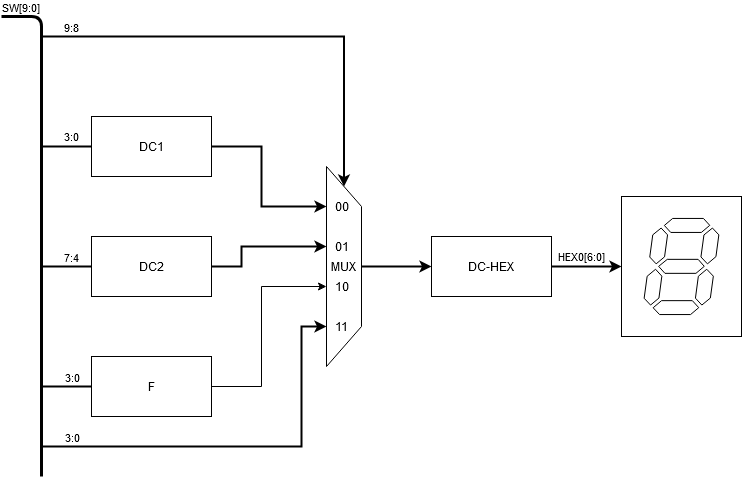
\includegraphics [width=1\textwidth] {images/lab_1/lab1_sch.png}
  \caption{Общая структурная схема проекта выполненной лабораторной работы.}
  %\label{lab1:pic1}
\end{figure}


\par{Описать на языке Verilog цифровое устройство, функционирующее согласно следующим принципам:}
\begin{enumerate}
  \item Ввод информации происходит с переключателей SW[9:0];
  \item SW[3:0] должны обрабатываться дешифратором «DC1», согласно индивидуальному заданию;
  \item SW[7:4] должны обрабатываться дешифратором «DC2», согласно индивидуальному заданию;
  \item Функция алгебры логики «F» должна принимать на вход сигналы SW[3:0].

  \item Реализовать дешифратор «DC-DEC», преобразующий число, представленное в двоичном коде в цифру, отображаемую на семисегментном индикаторе. Руководствоваться при этом нужно следующими соображениями:
    \begin{itemize}
      \item Семисегментный индикатор подключается к шине HEX0[6:0]
      \item Диоды на семисегментном индикаторе загораются при подаче на них низкого напряжения (0 - горит, 1 - не горит)
      \item Соответствие линий диодам семисегментного индикатора и пример кода дешифратора приведены ниже:
        \begin{figure}[H]
          \centering
          \def\svgwidth{\columnwidth}
          \includesvg{images/lab_1/7seg}
          \label{fig:decoder}
        \end{figure}

        \noindent
        \begin{minipage}{\linewidth}
          \lstinputlisting[caption={Пример описания дешифратора для семисегментного индикатора.}]{./code_examples/lab_1/dc_hex.v}
        \end{minipage}



    \end{itemize}
    \item С помощью мультиплексора «MUX» реализовать следующую схему подключения:
      \begin{itemize}
        \item Если SW[9:8] = 00, на дешифратор DC-DEC поступает выход DC1;
        \item Если SW[9:8] = 01, на дешифратор DC-DEC поступает выход DC2;
        \item Если SW[9:8] = 10, на дешифратор DC-DEC поступает выход логической функции F;
        \item Если SW[9:8] = 11, на дешифратор DC-DEC поступает SW[3:0].
      \end{itemize}
\end{enumerate}



\par{Выполнив описание модуля на языке Verilog необходимо построить временные диаграммы его работы с помощью САПР Altera Quartus.}
\par{Привязать входы модуля к переключателям SW отладочной платы, а выход к шине HEX0[6:0], получить прошивку для ПЛИС и продемонстрировать её работу.}


\section{Варианты индивидуальных заданий}


\begin{enumerate}
  
  \setlength\itemsep{1em}

  \item{
    \begin{itemize}
    \item Логика работы дешифратора DC1: \\
      Кодирует количество переключателей SW[3:0] в положении «0».
    \item Логика работы дешифратора DC2: \\ 
      Логическое "ИЛИ" сигналов с переключателей SW[7:4] с числом «0101».
    \item Функция f:\\
      $f = SW[0] || (SW[1] \oplus (SW[2] \& SW[3]))$
    \end{itemize}
  }

  \item{
    \begin{itemize}
    \item Логика работы дешифратора DC1: \\
      Кодирует количество сочетаний «01» на SW[3:0]
    \item Логика работы дешифратора DC2: \\ 
      Логическое "И" сигналов с переключателей SW[7:4] с числом «1101»
    \item Функция f:\\
      $f = (SW[0] \oplus  SW[1]) || (SW[2] \oplus  SW[3])$
    \end{itemize}
  }

    \item{
    \begin{itemize}
    \item Логика работы дешифратора DC1: \\
      Кодирует количество сочетаний «10» на SW[3:0]
    \item Логика работы дешифратора DC2: \\ 
      Логическое "НЕ" сигналов с переключателей SW[7:4]
    \item Функция f:\\
      $f = SW[0] \& SW[1] \& (\neg SW[2]) \& (\neg SW[3])$
    \end{itemize}
  }

    \item{
    \begin{itemize}
    \item Логика работы дешифратора DC1: \\
      Кодирует количество переключателей SW[3:0] в положении «1».
    \item Логика работы дешифратора DC2: \\ 
      Число с переключателей SW[7:4], сдвинутое на 1 двоичный разряд влево.
    \item Функция f:\\
      $f = (SW[0] || SW[1] || SW[2]) \& SW[3]$
    \end{itemize}
  }

    \item{
    \begin{itemize}
    \item Логика работы дешифратора DC1: \\
      Кодирует количество переключателей SW[3:0] в положении «0».
    \item Логика работы дешифратора DC2: \\ 
      Логическое "исключающее ИЛИ" сигналов с переключателей SW[7:4] с числом «0111».
    \item Функция f:\\
      $f = (\neg SW[0]) \oplus (\neg SW[1]) || (SW[2] \& SW[3])$
    \end{itemize}
  }

    \item{
    \begin{itemize}
    \item Логика работы дешифратора DC1: \\
      Кодирует количество сочетаний «01» на SW[3:0]
    \item Логика работы дешифратора DC2: \\ 
      Логическое "НЕ" сигналов с переключателей SW[7:4]
    \item Функция f:\\
      $f = (\neg SW[0]) || (\neg SW[1]) || (\neg SW[2]) || (\neg SW[3])$
    \end{itemize}
  }

    \item{
    \begin{itemize}
    \item Логика работы дешифратора DC1: \\
      Кодирует количество сочетаний «11» на SW[3:0]
    \item Логика работы дешифратора DC2: \\ 
      Логическое "И" сигналов с переключателей SW[7:4] с числом «1001»
    \item Функция f:\\
      $f = (SW[0] \& SW[1]) \oplus (SW[2] || SW[3])$
    \end{itemize}
  }

    \item{
    \begin{itemize}
    \item Логика работы дешифратора DC1: \\
      Число с переключателей SW[3:0]  - число 3 (десятичное).
    \item Логика работы дешифратора DC2: \\ 
      Логическое "исключающее ИЛИ" сигналов с переключателей SW[7:4] с числом «1000».
    \item Функция f:\\
      $f = ((\neg SW[0]) \& SW[1]) || SW[2] || SW[3]$
    \end{itemize}
  }

    \item{
    \begin{itemize}
    \item Логика работы дешифратора DC1: \\
      Число с переключателей SW[3:0], делённое на 2 без остатка.
    \item Логика работы дешифратора DC2: \\ 
      Логическое "И" сигналов с переключателей SW[7:4] с числом «1010»
    \item Функция f:\\
      $f = (SW[0] \oplus SW[3]) \& (SW[1] || SW[2])$
    \end{itemize}
  }

    \item{
    \begin{itemize}
    \item Логика работы дешифратора DC1: \\
      Кодирует количество сочетаний «010» на SW[3:0]
    \item Логика работы дешифратора DC2: \\ 
      Логическое "исключающее ИЛИ" сигналов с переключателей SW[7:4] с числом «0011».
    \item Функция f:\\
      $f = SW[0] || SW[1] \& SW[2] || SW[3]$
    \end{itemize}
  }



\end{enumerate}

\chapter{Лабораторная работа №3\\Регистры и счётчики} 

\par{Функции цифровых устройств, естественно, не сводятся к реализации разнообразных ФАЛ. Нам хотелось бы использовать цифровые устройства для обработки информации, вычислений. Но для осуществления этих возможностей нам недостаёт элемента памяти, который мог бы хранить промежуточные результаты. Ведь невозможно сделать калькулятор, если нет возможности сохранить вводимые числа и результат вычисления.}

\par{Элемент памяти — один из самых важных элементов цифровых устройств. Чтобы не делать ошибок при разработке цифровых устройств, необходимо понять место этого узла, его идею и инструменты языка \eng{Verilog}, связанные с ним.}

\par{Первый элемент памяти, который мы рассмотрим — это  \textbf{защелка} (англ. \eng{latch}).}

\par{Защелка является основой всех элементов памяти. Она состоит из двух элементов И-НЕ (или из двух элементов ИЛИ-НЕ, в зависимости от базиса, выбранного при проектировании), соединенных по следующей схеме:}

\begin{figure}[H]
	\centering
	\def\svgwidth{\columnwidth}
	\includesvg{RS_latch}
	\caption{Структура \eng{RS}-защелки}
\end{figure}

\par{У защелки два входа и два выхода. Входами являются сигналы \quotes{сброс} и \quotes{установка в единицу} или по-английски \quotes{reset} и \quotes{set}. В зависимости от элементов, из которых состоит защелка, полярность входных сигналов будет меняться. В базисе И-НЕ сброс и установка происходят, когда соответственно сигналы \eng{R} или \eng{S} находятся в нуле, поэтому их обозначают как \quotes{не-сброс} и \quotes{не-установка}, чтобы отразить этот факт. Выход защелки — это тот бит данных, который она хранит. Два выхода отличаются полярностью — один из них инвертирует хранимый бит. Ниже приведена таблица со всеми возможными комбинациями входных сигналов и временная диаграмма работы защелки.}

\begin{figure}[H]
\centering
\begin{tikztimingtable}[%
    timing/dslope=0.1,
    timing/.style={x=6ex,y=3ex},
    very thick,
    x=5ex,
    timing/rowdist=3ex,
    timing/name/.style={font=\sffamily\scriptsize},
]

	S  & 1L 4H \\
	R  & 3H 2L \\
	Q  & 3H 2L \\
\extracode
\begin{pgfonlayer}{background}
\draw [->,>=latex] (0,0ex) --  (30ex+1,0ex);
\draw [->,>=latex] (0,-3ex) -- (30ex+1,-3ex);
\draw [->,>=latex] (0,-6ex) -- (30ex+1,-6ex);
\draw [->,>=latex] (0,-6ex) -- (0,4ex);

\node [align=center,scale=0.6,text width=7ex] at (2ex, -8ex) {Установка в \quotes{1}};
\node [align=center,scale=0.6,text width=6ex] at (12ex,-8ex) {Хранение};
\node [align=center,scale=0.6,text width=6ex] at (24ex,-8ex) {Сброс в \quotes{0}};

\begin{scope}[semitransparent ,semithick]
\foreach \i in {6ex, 18ex} {
\draw[darkgray,dotted] (\i,4ex) -- (\i,-10ex);
}
%\vertlines[darkgray,dotted]{6ex,18ex}
\end{scope}
\end{pgfonlayer}
\end{tikztimingtable}
\caption{Временная диаграмма работы \eng{RS}-защелки}
\end{figure}

\par{Опишем защелку на языке \eng{Verilog}, опираясь на её структуру, которую мы рассмотрели выше. Нам понадобятся два входа, два выхода и два элемента И-НЕ, которые мы опишем с помощью операций И (оператор \&) и НЕ (оператор \textasciitilde).}

\lstinputlisting[caption={Описание \eng{RS}-защелки на языке \eng{Verilog HDL}}, ]{./code_examples/rs_latch.v}
		
\par{Элемент памяти нам, прежде всего, нужен для хранения данных. Для того, чтобы защелкой стало удобнее пользоваться, немного изменим схему подключения управляющих сигналов.}

\begin{figure}[H]
	\centering
	\def\svgwidth{\columnwidth}
	\includesvg{D_latch}
	\caption{Структура \eng{D}-защелки}
\end{figure}
		
\par{Защелка теперь будет работать следующим образом: при высоком уровне на входе \quotes{разрешить работу} (\qeng{enable}) данные со входа \quotes{данные} (\qeng{data}) будут проходить через защелку на выход, при низком уровне на входе \quotes{разрешить работу} защелка будет сохранять на выходе последнее значение со входа \quotes{данные}, которое было до переключения сигнала \quotes{разрешить работу}. Работа такой защелки показана на временной диаграмме ниже.}

\begin{figure}[H]
\centering
\begin{tikztimingtable}[%
    timing/dslope=0.1,
    timing/.style={x=6ex,y=3ex},
    very thick,
    x=5ex,
    timing/rowdist=4ex,
    timing/name/.style={font=\sffamily\scriptsize},
]

	EN & 1L 2H 2L \\
	D  & 3H 2L \\
	Q  & 1X 2H 2L \\
\extracode
\begin{pgfonlayer}{background}
\draw [->,>=latex] (0,0ex) --  (30ex+0.4,0ex);
\draw [->,>=latex] (0,-4ex) -- (30ex+0.4,-4ex);
\draw [->,>=latex] (0,-8ex) -- (30ex+0.4,-8ex);
\draw [->,>=latex] (0,-8ex) -- (0,4ex);
\node [scale=0.6] at (3ex, -9ex) {Хранение};
\node [scale=0.6] at (12ex,-9ex) {Запись};
\node [scale=0.6] at (24ex,-9ex) {Хранение};

\draw [->,thick] (-1.6,-1.9) to [out=-90,in=180] (-0.6,-3.4) to [out=0,in=90] (2.5ex,-4);
\node [align=center, above, text width= 10 ex, scale=0.8] at (-2.3,-1.9) {неизвестное значение};

\begin{scope}[semitransparent ,semithick]
\foreach \i in {6ex, 18ex} {
\draw[darkgray,dotted] (\i,4ex) -- (\i,-10ex);
}
%\vertlines[darkgray,dotted]{6ex,18ex}
\end{scope}
\end{pgfonlayer}
\end{tikztimingtable}
\caption{Временная диаграмма работы \eng{D}-защелки}
\end{figure}

\par{Как мы уже говорили, использовать структурные описания не всегда удобно. В большинстве случаев использовать поведенческое описание намного эффективнее. Поведенческое описание часто формулируется гораздо лаконичнее, и, так как его легче понять человеку, улучшается читаемость кода и уменьшается вероятность ошибок при его написании.}

\lstinputlisting[caption={Поведенческое описание \eng{D}-защелки на языке \eng{Verilog HDL}}, ]{./code_examples/d_latch.v}
		
\par{Если добавить к этой схеме еще две защелки, то можно привязать изменение \quotes{содержимого} защелки к переходу управляющего сигнала из \quotes{0} в \quotes{1}, то получим следующую структуру:}

\begin{figure}[H]
	\centering
	\def\svgwidth{\columnwidth}
	\includesvg{dff_struct}
	\caption{Структура \eng{D}-триггера}
\end{figure}
		
\par{Эту схему можно немного доработать, введя управляющие сигналы сброса, установки в единицу и разрешения работы. Упрощенно такая схема изображается следующим образом.}

\begin{figure}[H]
	\centering
	\def\svgwidth{\columnwidth}
	\includesvg{dff}
	\caption{Графическое обозначение \eng{D}-триггера}
\end{figure}
		
\par{Эта схема получила широчайшее применение в цифровой схемотехнике и называется \eng{d}-триггер (от слова \qeng{data} — данные). Ниже приведена временная диаграмма работы \eng{d}-триггера.}


\begin{figure}[H]
\centering
\begin{tikztimingtable}[%
    timing/dslope=0.1,
    timing/.style={x=3ex,y=2ex},
    very thick,
    x=3ex,
    timing/rowdist=4ex,
    timing/name/.style={font=\sffamily\scriptsize},
]
	CLK   & 3{c} N(C1) 2{c} N(C2) 2{c} N(c1) 2{c} N(c2) 2{c} N(C3) 2{c} N(C4) 2{c} N(c3) 2{c} N(c4) 2{c} N(c5) 2{c} N(c6) 2{c} N(c7) 2{c} N(c8) 2{c} N(c9) 2{c} N(c10) 1.5{c}\\
	D     & 1.5L N(D1) H N(D2) H N(d1) 1L N(d2) 1H N(D3) 1L N(D4) H N(d3) H N(d4) H N(d5) L N(d6) L N(d7) L N(d8) L N(d9) L N(d10) 0.5L\\
	EN    & 6.5H L N(E1) L N(E2) L N(E3) L N(E4) L N(E5) L N(e6) L N(E6) L N(E7) 0.5L\\
        S     & 12.5L N(S1) 0.5H 2L \\
	R     & 3L N(R1) 0.5H N(R2) H N(R3) 0.5H 10L\\
	Q     & 0.5X 2L 0.5H 2.5L 1H 6L 2.5H\\
\extracode

\draw [semithick, color=red]
(C1) ellipse (.1 and .2)
(C2) ellipse (.1 and .2)
(C3) ellipse (.1 and .2)
(C4) ellipse (.1 and .2) 
(D1) ellipse (.1 and .2)
(D2) ellipse (.1 and .2)
(D3) ellipse (.1 and .2)
(D4) ellipse (.1 and .2)
(E1) ellipse (.1 and .2)
(E2) ellipse (.1 and .2)
(E3) ellipse (.1 and .2)
(E4) ellipse (.1 and .2)
(E5) ellipse (.1 and .2)
(E6) ellipse (.1 and .2)
(E7) ellipse (.1 and .2)
(S1) ellipse (.1 and .2)
(R1) ellipse (.1 and .2)
(R2) ellipse (.1 and .2)
(R3) ellipse (.1 and .2);

\node [color=red,scale=.8] at (c1) {$\times$};
\node [color=red,scale=.8] at (c2) {$\times$};
\node [color=red,scale=.8] at (c3) {$\times$};
\node [color=red,scale=.8] at (c4) {$\times$};
\node [color=red,scale=.8] at (c5) {$\times$};
\node [color=red,scale=.8] at (c6) {$\times$};
\node [color=red,scale=.8] at (c7) {$\times$};
\node [color=red,scale=.8] at (c8) {$\times$};
\node [color=red,scale=.8] at (c9) {$\times$};
\node [color=red,scale=.8] at (c10) {$\times$};

\node [color=red,scale=.8] at (d1) {$\times$};
\node [color=red,scale=.8] at (d2) {$\times$};
\node [color=red,scale=.8] at (d3) {$\times$};
\node [color=red,scale=.8] at (d4) {$\times$};
\node [color=red,scale=.8] at (d5) {$\times$};
\node [color=red,scale=.8] at (d6) {$\times$};
\node [color=red,scale=.8] at (d7) {$\times$};
\node [color=red,scale=.8] at (d8) {$\times$};
\node [color=red,scale=.8] at (d9) {$\times$};
\node [color=red,scale=.8] at (d10) {$\times$};
\node [color=red,scale=.8] at (e6) {$\times$};

\draw [color=red,semithick,shorten >=.3ex,shorten <=.3ex] (C1) -- (D1);
\draw [color=red,semithick,shorten >=.3ex,shorten <=.3ex] (C2) -- (D2);
\draw [color=red,semithick,shorten >=.3ex,shorten <=.3ex] (C3) -- (D3);
\draw [color=red,semithick,shorten >=.3ex,shorten <=.3ex] (C4) -- (D4);

\begin{pgfonlayer}{background}
\draw [->,>=latex] (0,0ex) -- (\twidth+0.2,0ex);
\draw [->,>=latex] (0,-4ex) -- (\twidth+0.2,-4ex);
\draw [->,>=latex] (0,-8ex) -- (\twidth+0.2,-8ex);
\draw [->,>=latex] (0,-12ex) -- (\twidth+0.2,-12ex);
\draw [->,>=latex] (0,-16ex) -- (\twidth+0.2,-16ex);
\draw [->,>=latex] (0,-20ex) -- (\twidth+0.2,-20ex);
\draw [->,>=latex] (0,-20ex) -- (0,4ex);
\end{pgfonlayer}
\end{tikztimingtable}
\caption{Пример работы регистра}
\end{figure}



	
\par{Заметим, что сигнал \eng{C} называют \quotes{тактирующим} сигналом или \quotes{сигналом синхронизации}. Обычно в роли этого сигнала выступает сигнал от внешнего источника (чаще всего кварцевого резонатора) со стабильной частотой. А сами цифровые устройства, для работы которых необходим сигнал синхронизации, называют синхронными.}

\par{Сигнал синхронизации играет очень большую роль в цифровых устройствах. Прежде всего, он необходим для того, чтобы избежать непредсказуемого и нестабильного поведения триггеров в цифровых устройствах.}

\lstinputlisting[caption={Описание \eng{D}-триггера на языке \eng{Verilog HDL}}, ]{./code_examples/d_flipflop.v}
		
\par{В описании появилось новое ключевое слово \eng{posedge}. Оно используется только в списке чувствительности блока \eng{always} и означает событие перехода сигнала, имя которого стоит после этого ключевого слова, из состояния \quotes{0} в состояние \quotes{1}.}
		
		
\par{Ключевое слово \eng{posedge} было введено прежде всего для того, чтобы описывать схемы, содержащие триггеры. Ведь триггеры, как мы уже говорили, могут менять своё состояние только в момент положительного фронта (англ. \eng{positive edge}) сигнала синхронизации.}
		
		
\par{Добавление в список чувствительности события \eng{posedge rst} позволяет описать поведение триггера в момент асинхронного сброса: как только случается переход \eng{rst} из \quotes{0} в \quotes{1} срабатывает блок \eng{always} и проверка условия \kword{if} (\eng{rst}) дает положительный результат, триггер сбрасывается в \quotes{0}.}

\par{}

\par{Если объединить несколько триггеров в группу, то получится то, что в цифровой схемотехнике называют \quotes{регистр}.}

\lstinputlisting[caption={Описание регистра на языке \eng{Verilog HDL}}, ]{./code_examples/register.v}
		
\par{Элементы памяти позволяют нам сохранять информацию для дальнейшей обработки или хранить готовый результат вычисления, хранить промежуточные результаты.}

\par{Запомните описание регистра. Оно используется при проектировании практически любого цифрового устройства с помощью \eng{Verilog}.}	

\par{Необходимо отметить важную концепцию языка \eng{Verilog}. \textbf{Переменные типа \eng{reg} могут быть изменены только в пределах одного блока \eng{always}. Переменные доступны для проверки в любом из блоков, но изменять их значение можно только в одном из них.}}	

\lstinputlisting[caption={Пример присвоения значения переменной а разных блоках \eng{always} на языке \eng{Verilog HDL}}, ]{./code_examples/error_example_2.v}

\par{Одной из простейших, и в тоже время широко распространённой, цифровой схемой на основе регистров является счётчик.}

\par{Счётчик считает количество тактов, которое прошло с момента его обнуления.}
		
\par{Такая простая схема, тем не менее, используется практически в каждом цифровом устройстве. Как будет показано дальше, счётчик легко можно доработать таким образом, чтобы отсчитывались не такты, а какие-то события. Например, событиями могут быть: нажатие кнопки, принятие пакета данных, срабатывание датчика, выполнение какого-то условия (периодическое) и другое.}		

\par{}

\par{Итак, для того чтобы реализовать счетчик нам понадобится регистр и сумматор. Причем сумматор будет складывать значение, хранящееся в регистре с константой (в нашем случае единицей) а результат сложения будет поступать на вход регистра.}		
		
\par{}

\par{В результате получим следующую схему:}

\begin{figure}[H]
	\centering
	\def\svgwidth{\columnwidth}
	\includesvg{counter}
	\caption{Структура восьмибитного счетчика}
\end{figure}
		
\par{На временной диаграмме ниже хорошо видно как работает счётчик:}



\begin{figure}[H]
\centering
\begin{tikztimingtable}[%
    timing/dslope=0.1,
    timing/.style={x=3ex,y=2ex},
    very thick,
    x=3ex,
    timing/rowdist=3ex,
    timing/name/.style={font=\sffamily\scriptsize},
]
	CLK   & 18{c} \\
	R     & 1L 0.5H 7.5L \\
	EN     & 2L 3H 2L 2H\\
        count & 1X 2D{0} 1D{1} 1D{2} 3D{3} 1D{4} \\
\extracode
\begin{pgfonlayer}{background}
\draw [->,>=latex] (0,0ex) -- (\twidth+0.2,0ex);
\draw [->,>=latex] (0,-3ex) -- (\twidth+0.2,-3ex);
\draw [->,>=latex] (0,-6ex) -- (\twidth+0.2,-6ex);
\draw [->,>=latex] (0,-9ex) -- (\twidth+0.2,-9ex);
\draw [->,>=latex] (0,-9ex) -- (0,3ex);
\end{pgfonlayer}
\end{tikztimingtable}
\caption{Пример работы регистра}
\end{figure}


	
\par{Опишем поведение такого счётчика на \eng{Verilog}.}

\lstinputlisting[caption={Описание восьмиитного счетчика на языке \eng{Verilog HDL}}, ]{./code_examples/counter_8bit.v}
		
\par{Для того чтобы можно было подсчитывать события, а не переходы сигнала синхронизации из \quotes{0} в \quotes{1} понадобится ввести еще одну схему. Её смысл и назначение заключается в следующем: нам необходимо из асинхронного события получить синхронный сигнал единичной длительности. Тогда, подавая такой сигнал на вход \eng{enable} счётчика, мы сможем считать количество произошедших событий.}
		
\par{Ниже представлена схема, позволяющая сделать это:}

\begin{figure}[H]
	\centering
	\def\svgwidth{\columnwidth}
	\includesvg{register_2}
	\caption{Структура регистра на \eng{D}-триггерах}
\end{figure}

\begin{figure}[H]
\centering
\begin{tikztimingtable}[%
    timing/dslope=0.1,
    timing/.style={x=3ex,y=2ex},
    very thick,
    x=3ex,
    timing/rowdist=3ex,
    timing/name/.style={font=\sffamily\scriptsize},
]
	CLK & 22{c} \\
	D   & 1.5L 4.5H 5L \\
	Q   & 3.5L 1H 6.5L \\
\extracode
\begin{pgfonlayer}{background}
\draw [->,>=latex] (0,0ex) --  (\twidth+0.2,0ex);
\draw [->,>=latex] (0,-3ex) -- (\twidth+0.2,-3ex);
\draw [->,>=latex] (0,-6ex) -- (\twidth+0.2,-6ex);
\draw [->,>=latex] (0,-6ex) -- (0,3ex);
\end{pgfonlayer}
\end{tikztimingtable}
\caption{Пример работы регистра}
\end{figure}

\par{Естественно такая схема работает только тогда, когда входной сигнал изменяется с частотой меньшей, чем частота синхронизации.}

\par{Сигнал \eng{out} в таком случае подключается к входу \eng{enable} счётчика.}		
		
\section{Задание лабораторной работы}

\par{Описать на языке \eng{Verilog} цифровое устройство, функционирующее согласно следующим принципам:
\begin{enumerate}[noitemsep,topsep=0pt, after=\vspace{2pt}]
  \item Ввод информации происходит с переключателей \eng{SW}[9:0] и кнопок \eng{KEY}[0], \eng{KEY}[1]. Внешний источник сигнала синхронизации: \eng{CLK}50;
  \item \eng{KEY}[1] должна функционировать как общий асинхронный сброс устройства;
  \item При нажатии на \eng{KEY}[0] записывать данные с \eng{SW}[9:0] в десятиразрядный регистр;
  \item Содержимое десятиразрядного регистра выводить на \eng{LEDR}[9:0];
  \item При нажатии на \eng{KEY}[0] увеличивать 8-ми разрядный счётчик нажатий на 1, если произошло событие, указанное в индивидуальном задании студента;
  \item Содержимое счётчика выводить в шестнадцатеричной форме на \eng{HEX}0 и \eng{HEX}1 (цифры с 0 до 9 и буквы \eng{A}, \eng{B}, \eng{C}, \eng{D}, \eng{E}, \eng{F})
\end{enumerate}}
		
\par{Выполнив описание модуля на языке \eng{Verilog} необходимо построить временные диаграммы его работы с помощью САПР \eng{Altera Quartus}.}		
		
\par{Привязать входы модуля к переключателям \eng{SW}, отладочной платы, а выход к шине \eng{HEX}0[6:0], получить прошивку для ПЛИС и продемонстрировать её работу.}
		
\section{Пример индивидуального задания}

\par{Событием является наличие 3 и более единиц на SW[9:0] в момент записи в регистр.}

\lstinputlisting[caption={Решение индивидуального задания (фрагмент кода лабораторной работы)}, ]{./code_examples/task_solution_2.v}
		
\section{Вопросы к защите лабораторной работы}

\begin{enumerate}[noitemsep,topsep=0pt, after=\vspace{2pt}]
  \item Какие элементы памяти вы изучили в данной лабораторной работе?
  \item Чем отличается \eng{RS}-защелка от \eng{D}-защелки?
  \item Какие входы могут быть у триггера? Перечислите все и назовите их функции.
  \item Какие блоки вашего цифрового устройства синхронные? Какие нет? Почему?
  \item Какой фрагмент вашего кода описывает вывод значения счетчика на семи сегментный индикатор? Как называется эта цифровая схема?
  \item Продемонстрируйте код реализующий индивидуальное задание.
  \item Покажите в коде лабораторной код счётчика.
  \item Что такое сигнал синхронизации?
\end{enumerate}

\chapter{Лабораторная работа №3\\Секундомер} 

\par{В прошлых лабораторных работах мы изучили базовые строительные блоки цифровых устройств. Теперь у нас уже достаточно знаний для реализации несложного, но функционально законченного цифрового устройства.}

\par{В данной лабораторной работе мы познакомимся с процессом проектирования полноценного цифрового устройства на примере разработки простого секундомера. Мы подробно, поэтапно, рассмотрим процесс проектирования, проиллюстрировав каждый этап графической схемой.}

\par{Для эффективного проектирования любого цифрового устройства нужно придерживаться некоторой \quotes{канвы} проектирования. Это поможет не запутаться и последовательно разобраться с вопросами, возникающими в ходе проектирования.}

\par{\textbf{Начинать проектирование любого цифрового устройства следует с определения входов и выходов.} Нужно понять, какие данные будут входными для проектируемого устройства, и какие данные нам надо выработать и подать на выход.}

\vspace{4mm}
\par{В случае секундомера справедливы такие рассуждения:}
\par{Чтобы управлять работой секундомера нам понадобятся два входа: \quotes{старт/стоп} и \quotes{сброс}.}
\par{Для отображения времени можно воспользоваться семисегментными индикаторами. Значит, для управления каждым из них понадобится семибитная шина, которая будет выходом нашего устройства.}
\par{Для отображения времени выделим 2 индикатора для отображения количества прошедших секунд и 2 индикатора для отображения количества прошедших десятых и сотых долей секунды.}
\par{Значит выходом секундомера будут четыре семибитные шины для управления индикаторами.}
\par{В основе секундомера лежит счётчик. Работая, секундомер отсчитывает время, считая количество пришедших импульсов сигнала синхронизации, частота которого заранее известна.}
\par{Т.е. нам потребуется сигнал синхронизации со стабильной частотой.}
\vspace{4mm}

\par{Больше никаких входов и выходов не требуется.}
\par{Общая схема на данный момент выглядит так:}

\begin{figure}[H]
	\centering
	\def\svgwidth{\columnwidth}
	\includesvg{images/lab_3/blackbox}
	\caption{Общая схема секундомера}
\end{figure}

\par{Начнём описывать модуль на языке \eng{Verilog}:}

\lstinputlisting[caption={Описание входов и выходов секундомера}, ]{./code_examples/lab_3/stopwatch_module.v}

\par{Теперь приступим к описанию \quotes{внутренностей} модуля.}

\par{Чтобы реализовать секундомер, нам необходимо отсчитывать время.}

\par{Для отсчёта времени в цифровых устройствах считают количество прошедших импульсов синхронизации (тактов). Так как тактовые импульсы генерируются кварцевым генератором со стабильной, известной нам, частотой, то мы можем рассчитать количество импульсов, которое соответствует заданному времени.}

\par{Например, если в устройстве установлен кварцевый генератор на 26 МГц, то одной секунде соответствует 26 миллионов тактовых импульсов, а одной сотой секунды соответствует 260 тысяч тактовых импульсов.}

\par{Для того, чтобы отсчитать это количество импульсов подходит единственный из известных нам \quotes{строительных блоков} - счётчик:}

\begin{figure}[H]
	\centering
	\def\svgwidth{\columnwidth}
	\includesvg{images/lab_3/counter}
	\caption{Структура счетчика}
\end{figure}


\par{Как мы уже говорили, счётчик состоит из регистра и сумматора. Чтобы счётчик циклически отсчитывал одну сотую секунды его необходимо обнулить после того, как он отсчитает 260 тысяч тактовых импульсов. В этот же момент нужно выработать сигнал для остальной схемы, что прошла одна сотая секунды.}

\par{Из всех цифровых блоков, которые мы рассмотрели, для реализации задачи сравнения текущего значения счётчика с константой подходит только компаратор. На один из входов компаратора подадим текущее значение счётчика, а на другой вход - константу 260 000.}

\begin{figure}[H]
	\centering
	\def\svgwidth{\columnwidth}
	\includesvg{images/lab_3/count_comp}
	\caption{Структура счетчика с компаратором}
\end{figure}

\par{Пока значения на входах компаратора будут отличаться, на выходе компаратора будет значение \quotes{0}. Когда значения будут равны, компаратор изменит выход с \quotes{0} на \quotes{1}, это и будет признак того, что прошло 0.01 секунды. Для того, чтобы можно было эффективно использовать сигнал \quotes{прошло 0.01с}, этот сигнал должен иметь длительность равную 1 такту.}

\par{Этот же сигнал мы будет использовать для управления сбросом счётчика.}

\par{Итак, счётчик должен после достижения значения 260 000 принять значение \quotes{0}, но переход должен случиться, как и все остальные переходы, в момент перехода тактового сигнала из \quotes{0} в \quotes{1}.}

\par{Сброс, отвечающий таким условиям, называется \quotes{синхронный сброс}.}

\par{Посмотрите, как будет выглядеть на временной диаграмме как будет работать счётчик если выход компаратора, подключить как сигнал синхронного сброса:}

\begin{figure}[H]
\centering
\begin{tikztimingtable}[%
    timing/dslope=0.1,
    timing/.style={x=5ex,y=2ex},
    very thick,
    x=3ex,
    timing/rowdist=3.3ex,
    timing/name/.style={font=\sffamily\scriptsize},
]

	& 16{c} \\
	& 0.5D{} D{259997} D{259998} D{259999} D{0} D{1} D{2} D{3} 0.5D{}\\
	& 2.5L 1H 4.5L\\
\extracode
\begin{pgfonlayer}{background}
\node [align=center,scale=0.6,text width=26ex] at (-8ex, -6ex) {Выход компаратора, подключенный в виде синхронного сброса};
\begin{scope}[semitransparent ,semithick]
\end{scope}
\end{pgfonlayer}
\end{tikztimingtable}
\caption{Временная диаграмма работы счётчика с синхронным сбросом}
\end{figure}

\par{А так выглядит временная диаграмма, если подключить выход компаратора к входу асинхронного сброса триггера:}

\begin{figure}[H]
\centering
\begin{tikztimingtable}[%
    timing/dslope=0.1,
    timing/.style={x=5ex,y=2ex},
    very thick,
    x=3ex,
    timing/rowdist=3.3ex,
    timing/name/.style={font=\sffamily\scriptsize},
]
	& 16{c} \\
	& 0.5D{} D{259996} D{259997} D{259998} 0.3D{} 0.7D{0} D{1} D{2} D{3}0.5D{}\\
	& 3.5L 0.3H 4.2L\\
\extracode
\begin{pgfonlayer}{background}
\node [align=center,scale=0.6,text width=26ex] at (-8ex, -6ex) {Выход компаратора, подключенный в виде асинхронного сброса};
\draw [->,thick] (12ex,-8ex) to [out=50,in=190] (16ex,-5ex) to [out=10,in=-100] (18.5ex,-3.3ex);
\node [align=center,below,scale=0.6,text width=10ex] at (12ex,-8ex) {259999};
\begin{scope}[semitransparent ,semithick]
\end{scope}
\end{pgfonlayer}
\end{tikztimingtable}
\caption{Временная диаграмма работы счётчика с асинхронным сбросом}
\end{figure}

\par{Выход компаратора, установившись в единицу, моментально сбросит счётчик и, так как значение счётчика изменилось, а значит, изменился и один из входов компаратора, выход компаратора сразу же перейдет в значение \quotes{0}.}

\par{Обратите внимание, что длительность сигнала с выхода компаратора должна быть равна одному такту. Ведь в дальнейшем нам необходимо будет считать события \quotes{прошла одна сотая секунды}, а значит подготовить сигнал единичной длительности, который соответствует этому событию (см. лабораторную работу №2).}

\par{Сигнал с компаратора в случае, когда он подключен в виде синхронного сброса, полностью удовлетворяет этому условию, а значит нам не придется в дальнейшем вводить новые фрагменты схемы.}

\par{Как реализовать синхронный сброс в цифровом устройстве?}

\par{Для этого можно использовать мультиплексор. Схема будет выглядеть следующим образом:}

\begin{figure}[H]
	\centering
	\def\svgwidth{\columnwidth}
	\includesvg{images/lab_3/sync_reset}
	\caption{Схема реализации синхронного сброса}
\end{figure}

\par{Если подключить \eng{sync\_reset} к выходу компаратора, то когда счётчик достигнет порогового значения, выход компаратора изменится и переключит мультиплексор. Теперь на выход мультиплексора будет подаваться \quotes{0}. Этот сигнал будет поступать на вход триггера, но запись нового значения произойдет только во время положительного фронта сигнала синхронизации.}

\par{Для общего сброса секундомера при нажатии кнопки \quotes{сброс} как раз можно воспользоваться входом асинхронного сброса регистра. Ведь при нажатии кнопки \quotes{сброс} можно обнулять регистр мгновенно.}

\par{Теперь надо выбрать правильный сигнал управления работой счётчика - сигнал разрешения работы (\eng{Enable}, \eng{EN}). Ведь счётчик должен начинать считать после нажатия кнопки \quotes{старт/стоп}, а после её повторного нажатия должен останавливаться.}

\par{Для управления работой счётчика можно использовать сигнал, который будет единицей, пока счётчик должен работать и нулём, если отсчёт времени остановлен. Как раз такой сигнал можно подать на вход разрешения работы регистра. Назовём этот сигнал \qeng{device\_running}.}

\par{Посмотрите, как выглядит остановка и запуск счётчика в таком случае:}

\begin{figure}[H]
\centering
\begin{tikztimingtable}[%
    timing/dslope=0.1,
    timing/.style={x=5ex,y=2ex},
    very thick,
    x=3ex,
    timing/rowdist=3.3ex,
    timing/name/.style={font=\sffamily\scriptsize},
]
				& 16{c} \\
	\eng{device\_running}	& 2.5H 3L 2.5H\\
	Значение счетчика	& 0.5D{} D{19157} D{19158} 4D{19159} D{19160} 0.5D{}\\
\extracode
\end{tikztimingtable}
\caption{Временная диаграмма работы сигнала \eng{device\_running}}
\end{figure}

\par{К проектированию и описанию схемы, которая вырабатывала бы сигнал \qeng{device\_running}, мы вернемся позднее.}

\par{Стоит обратить внимание на следующий момент: что будет, если счётчик остановить в тот момент времени, когда его значение стало равно 259999?}

\par{Взгляните на временную диаграмму:}

\begin{figure}[H]
\centering
\begin{tikztimingtable}[%
    timing/dslope=0.1,
    timing/.style={x=5ex,y=2ex},
    very thick,
    x=3ex,
    timing/rowdist=3.3ex,
    timing/name/.style={font=\sffamily\scriptsize},
]

				& 16{c} \\
	\eng{device\_running}	& 2.5H 5.5L\\
				& 0.5D{} D{259997} D{259998} 5.5D{259999}\\
	Выход компаратора	& 2.6L 5.4H \\
\extracode
\end{tikztimingtable}
\caption{Временная диаграмма работы счетчика}
\end{figure}

\par{Для того чтобы не допустить такого поведения, можно немного изменить условие, запрещающее работу счётчика. Теперь мы будем дополнительно проверять сигнал с компаратора. И если счётчик в данный момент равен 259999, то запретить его работу будет невозможно.}

\par{Для решения этой задачи подойдет вентиль \quotes{или}. Условие будет таким: \quotes{работа разрешена, если сигнал \qeng{device\_running} равен единице \textbf{ИЛИ} когда текущее значение счётчика равно 259999}.}

\par{Теперь схема счётчика выглядит следующим образом:}

\begin{figure}[H]
	\centering
	\def\svgwidth{\columnwidth}
	\includesvg{images/lab_3/pulse_counter}
	\caption{Схема счетчика тысячных долей секунды}
\end{figure}

\par{Когда мы представили схему в виде набора цифровых блоков, мы можем описать её поведение на языке \eng{Verilog}:}

\lstinputlisting[caption={Описание счетчика тактовых импульсов на языке \eng{Verilog}}, ]{./code_examples/lab_3/pulse_counter.v}

\par{Теперь, когда у нас есть счетчик, отсчитывающий такты и сигнализирующий о том, что прошла сотая доля секунды, мы можем отсчитывать сотые доли секунды.}

\par{Перед нами встаёт выбор.}

\par{Первый вариант – отсчитывать количество прошедших сотых долей секунды единственным счётчиком. Значение этого счётчика мы можем дешифрировать, чтобы выделить из него количество единиц, десятков, сотен и тысяч прошедших долей секунды, чтобы подать эти значения на дешифраторы семисегментных индикаторов:}

\begin{figure}[H]
	\centering
	\def\svgwidth{\columnwidth}
	\includesvg{images/lab_3/timer_struct_1}
	\caption{Схема секундомера с дешифраторами разрядов}
\end{figure}

\par{Второй вариант – использовать отдельные счётчики для сотых долей секунды, десятых долей секунды, целых секунд и десятков секунд.}

\par{Т.е. первый счетчик подсчитывает количество прошедших сотых долей секунды от 0 до 9, и, затем обнуляется, вырабатывая сигнал \quotes{прошла десятая доля секунды}. Следующий счётчик, точно также считает уже десятые доли и вырабатывает сигнал \quotes{прошла одна секунда} и так далее.}

\begin{figure}[H]
	\centering
	\def\svgwidth{\columnwidth}
	\includesvg{images/lab_3/timer_struct_2}
	\caption{Схема секундомера со счётчиками разрядов}
\end{figure}

\par{Второй вариант для нас проще в реализации, компактнее, удобнее и понятнее.}

\par{Поэтому выберем именно его.}

\par{В качестве счётчиков подойдет уже описанная нами схема для подсчёта тактов, но с небольшими правками.}

\par{Счетчики подойдут нам потому, что функция их идентична – подсчёт событий с ограничением диапазона. Изменить нужно будет только разрядность счётчика с 16 на 4 и верхнюю границу счёта с 260000 на 9. Тогда счётчик будет выдавать признак переполнения (достижения границы отсчёта, когда его значение будет становиться) девяткой.}

\par{Еще одним моментом, о котором нужно позаботиться – длительность выходного сигнала.}

\par{Пока счётчик считал такты, его значение менялось каждый такт. Компаратор просто не мог принять значение 1 более чем на один такт. Теперь ситуация выглядит следующим образом:}

\begin{figure}[H]
\centering
\begin{tikztimingtable}[%
    timing/dslope=0.1,
    timing/.style={x=3.5ex,y=2ex},
    very thick,
    x=3ex,
    timing/rowdist=3.3ex,
    timing/coldist=2pt,  
    timing/name/.style={font=\sffamily\scriptsize},
]
	& 11{c} 2{0.5c} 11{c} \\
	& 0.5D{} D{[scale=0.7]{259997}} D{[scale=0.7]{259998}} D{[scale=0.7]{259999}} D{[scale=0.7]{0}} 1D{[scale=0.7]{1}} 0.5D{} D{[scale=0.7]{259997}} D{[scale=0.7]{259998}} D{[scale=0.7]{259999}} D{[scale=0.7]{0}} D{[scale=0.7]{1}} 0.5D{}\\
	& 2.5L 1H 4.5L 1H 2.5L\\
	& 3.5D{[scale=0.7]{8}} 2D{[scale=0.7]{9}} 3.5D{[scale=0.7]{9}} 2.5D{[scale=0.7]{0}} \\
	& 3.5L 5.5H 2.5L\\
	& 8L 1H 2.5L\\
\extracode
\draw[fill=white,color=white] (20ex,-19ex) rectangle (18.8ex,4ex);
\begin{pgfonlayer}{background}
\node [align=right,scale=0.7,text width=22ex] at (-10ex, -3ex) {Счетчик тактов};
\node [align=right,scale=0.7,text width=22ex] at (-10ex, -6ex) {\quotes{Прошла 0.01с}};
\node [align=right,scale=0.7,text width=22ex] at (-10ex, -9ex) {Счетчик сотых долей};
\node [align=right,scale=0.7,text width=22ex] at (-10ex, -12ex) {Выход компаратора счетчика сотых долей};
\node [align=right,scale=0.7,text width=22ex] at (-10ex, -15ex) {\quotes{Прошла 0.1с}};
\draw [very thick, color=black] (20.15ex,4ex) -- (20.15ex,-19ex);
\draw [very thick, color=black] (18.65ex,4ex) -- (18.65ex,-19ex);
\end{pgfonlayer}
\end{tikztimingtable}
\caption{Временная диаграмма работы секундомера}
\end{figure}

\par{Счетчик будет переключаться каждую 0,01 секунды, 0,1 секунды ,1 секунду или 10 секунд. И выход компаратора будет устанавливаться в 1 на всё время, которое потребуется для переключения счётчика из 9 в ноль. Т.е. в случае счётчика сотых долей секунды потребуется 259999 тактов.}

\par{Как выделить из всего времени, пока счётчик имеет значение \quotes{9} сигнал длительностью в один такт, который возникает в нужный момент времени? На временной диаграмме этот сигнал отмечен как \quotes{прошла 0,1с.}

\par{Сигнал \quotes{прошла 0,1с} можно получить из сигналов, представленных на временной диаграмме следующим образом: \quotes{прошла 0,1с} правда, когда выход компаратора равен единице \textbf{И} \quotes{прошла 0,01с}.}

\par{Схема счётчика практически не изменилась:}

\begin{figure}[H]
	\centering
	\def\svgwidth{\columnwidth}
	\includesvg{images/lab_3/hundredth_counter}
	\caption{Схема счётчика сотых долей секунды}
\end{figure}

\par{Скорректируем описание её работы на \eng{Verilog}:}

\lstinputlisting[caption={Описание счетчика сотых долей секунды на языке \eng{Verilog}}, ]{./code_examples/lab_3/hundredth_counter.v}

\par{Счётчики десятых долей секунды, целых секунд и десятков секунд устроены абсолютно также. В описаниях изменятся только названия сигналов и регистров. Единственное в чем необходимо быть внимательным – это подключение сигналов. Для правильного подключения надо свериться со схемой, которую мы выбрали ранее.}

\par{Теперь вернёмся к вопросам, которые мы отложили ранее.}

\par{В нашем устройстве пока нет описания схемы, которая вырабатывает сигнал \qeng{device\_running}. Сигнал должен управляться кнопкой, поэтому как мы уже говорили в лабораторной работе №2, потребуется схема, синхронизирующая сигнал, поступающий с кнопки, с внутренним сигналом \eng{clk} (тактовые импульсы).}

\par{Также сразу выделим из всего нажатия признак того, что кнопка была нажата, так, чтобы по длительности этот признак был равен одному такту.}

\par{Тогда схема будет абсолютно такой же, как и в лабораторной работе №2 и будет выглядеть следующим образом:}

\begin{figure}[H]
	\centering
	\def\svgwidth{\columnwidth}
	\includesvg{images/lab_2/register}
	\caption{Схема выработки синхронного импульса из асинхронного события}
\end{figure}

\par{Поведение такой схемы описывается на языке \eng{Verilog} следующим образом:}

\lstinputlisting[caption={Описание схемы синхронизации на языке \eng{Verilog}}, ]{./code_examples/lab_3/button_syncroniser.v}

\par{Эта схема и её описание подробно рассмотрены в лабораторной работе №2}

\par{Теперь нам нужно построить схему, которая по нажатию кнопки переключала бы сигнал \quotes{device\_running} из \quotes{0} в \quotes{1} и из \quotes{1} в \quotes{0}.}

\par{Что нам понадобится? Триггер, чтобы хранить значение \qeng{device\_running}. Чтобы менять значение на противоположное надо знать противоположное значение, значит, нужен инвертор. Событие должно случаться по сигналу \qeng{button\_was\_pressed}, а значит речь, скорее всего, идет о входе разрешения работы триггера.}

\par{Немного подумав над этими вводными, нетрудно составить следующую схему:}

\begin{figure}[H]
	\centering
	\def\svgwidth{\columnwidth}
	\includesvg{images/lab_3/device_stopped}
	\caption{Схема переключения сигнала \qeng{device\_running}}
\end{figure}

\par{Временная диаграмма, которая соответствует работе этого устройства:}

\begin{figure}[H]
\centering
\begin{tikztimingtable}[%
    timing/dslope=0.1,
    timing/.style={x=5ex,y=2ex},
    very thick,
    x=3ex,
    timing/rowdist=3.3ex,
    timing/name/.style={font=\sffamily\scriptsize},
]
					& 15{c} \\
	\eng{button\_was\_pressed}	& 1.5L 1H 3L 1H 1L\\
	\eng{device\_running}		& 2.5L 4H 1L\\
\extracode
\end{tikztimingtable}
\caption{Временная диаграмма переключения сигнала \qeng{device\_running}}
\end{figure}

\par{Описание поведения этой схемы на \eng{Verilog} также не представляет сложности. Выполните его самостоятельно.}

\par{Теперь приведем полное описание секундомера (за исключением схемы, вырабатывающей сигнал \qeng{device\_running}), выполненное на языке \eng{Verilog}:}

\lstinputlisting[caption={Описание секундомера на языке \eng{Verilog}}, ]{./code_examples/lab_3/stopwatch.v}

\section{Задание лабораторной работы:}


\begin{enumerate}[noitemsep,topsep=0pt, after=\vspace{2pt}]

	\item{Изучить разработку к лабораторной работе.}

	\item{Самостоятельно выполнить описание схемы, вырабатывающей сигнал \qeng{device\_running}.}

	\item{Выполнить синтез и моделирование работы счётчика.}

	\item{Продемонстрировать в результатах моделирования фрагменты временных диаграмм, приведенных в заработке.}

	\item{Изучить работу устройства, реализованного в ПЛИС учебного стенда.}

\end{enumerate}

%\par{Подготовить ответы на вопросы к защите лабораторной работы.}

%\section{Вопросы к защите лабораторной работы}

%\par{*in progress*}
\chapter{Лабораторная работа №6\\Контроллер \eng{PS/2} для клавиатуры} 

\par{Для успешного применения цифровых устройств в реальности важно обеспечить их взаимодействие с внешним миром. Для этого существуют внешние интерфейсы для обмена информацией с другими устройствами и приборами. Внешние интерфейсы имеют различное функциональное назначение и спецификацию. Например, раньше для подключения клавиатуры и мыши использовался интерфейс \eng{PS/2}. Один с самых простых способов подключения устройств ввода-вывода.}

\vspace{4mm}

\par{Давайте изучим протокол и реализацию интерфейса \eng{PS/2}.}

\par{Интерфейс \eng{PS/2} сточки зрения соединения представляет собой два провода \kword{Clock} и \kword{Data}. По \kword{Clock} передаются синхроимпульсы, а по \kword{Data} предаются данные. На рисунке пример одной транзакции обмена.}

\begin{figure}[H]
	\centering
	\def\svgwidth{\columnwidth}
	\includesvg{images/lab_6/diag}
	\caption{Передача данных по протоколу PS/2}
\end{figure}

\par{Структура транзакции похожа на \eng{UART} и состоит из:}
  \begin{enumerate}[noitemsep,topsep=0pt, after=\vspace{2pt}]
    \item старт бит – всегда ноль;
    \item 8 бит данных;
    \item бит четности, равен 1 если количество единиц в данных четно и 0 если нечетно;
    \item стоп бит – всегда единица.
  \end{enumerate}

\par{Данные на линию выставляются, когда \kword{Clock} равен \textbf{1} и считываются, когда \kword{Clock} равен \textbf{0}. На практике данные обычно выставляются по положительному фронту и считываются по отрицательному.}

\par{Частота сигнала \kword{Clock} примерно 10-16.7кГц. Время от фронта сигнала \kword{Clock} до момента изменения сигнала \kword{Data} не менее 5 микросекунд.}

\vspace{4mm}

\par{Транзакции разделяются на два вида:}
  \begin{enumerate}[noitemsep,topsep=0pt, after=\vspace{2pt}]
    \item От устройства к контроллеру;
    \item От контроллера к устройству.
  \end{enumerate}

\par{На примере клавиатуры.}
  \begin{enumerate}[noitemsep,topsep=0pt, after=\vspace{2pt}]
    \item Клавиатура посылает на контроллер восьмибитный код нажатой клавиши;
    \item Контроллер посылает на клавиатуру команды управления. Такие как, команды сброса, выключения светодиодов.
  \end{enumerate}

\begin{figure}[H]
	\centering
	\def\svgwidth{\columnwidth}
	\includesvg{images/lab_6/diag}
	\caption{Передача восьмибитного пакета данных}
\end{figure}

\par{При транзакции от устройства (клавиатуры) к контроллеру сигналы на линиях \kword{Clock} и \kword{Data} генерирует устройство. Контроллер выступает в роли приемника считывая данные по отрицательному фронту \kword{Clock}.}

\par{При передаче в обратную сторону команд от контроллера к клавиатуре или мыши протокол отличается от описанного выше.}

\par{Последовательность обмена другая:}
  \begin{enumerate}[noitemsep,topsep=0pt, after=\vspace{2pt}]
    \item контроллер опускает сигнал \kword{Clock} в ноль на время примерно 100 микросекунд;
    \item контроллер опускает сигнал \kword{Data} в ноль формируя старт бит;
    \item контроллер отпускает сигнал \kword{Clock} в логическую единицу, клавиатура фиксирует старт бит;
    \item далее клавиатура генерирует сигнал \kword{Clock}, а хост контроллер подает передаваемые биты;
    \item после того, как контроллер передал все свои биты, включая бит четности и стоп бит, клавиатура посылает последний бит «ноль», который является подтверждением приема.
  \end{enumerate}

\begin{figure}[H]
	\centering
	\def\svgwidth{\columnwidth}
	\includesvg{images/lab_6/diag_r}
	\caption{Распределение управления между контроллером и устройством}
\end{figure}

\par{Поскольку одним сигналом управляют два устройства, то довольно трудно понять, кто в какой момент времени управляет сигналом. По этому, диаграмма нарисована двумя цветами. Красный цвет – сигнал управляется контроллером, а синий – сигнал управляется устройством.}

\vspace{4mm}

\par{Давайте выясним какие коды же коды передает клавиатура для каждой клавиши.}

\par{Ниже приведена таблица кодов для клавиш. Каждой клавише соответствует код генерируемый при нажатии и код генерируемый при деактивации. Коды состоящие из нескольких байтов предаются в нескольких подряд идущих транзакций.}

\vspace{4mm}

\begin{center}
  \begin{tabular}{ | l | l | l | l | l | l | }
    \hline
	    \kword{KEY} & \kword{MAKE} & \kword{BREAK} & \kword{KEY} & \kword{MAKE} & \kword{BREAK} \\ \hline
	    A & 1C & F0,1C & R ALT & E0,11 & E0,F0,11  \\ \hline
	    B & 32 & F0,32 & APPS  & E0,2F & E0,F0,2F  \\ \hline
	    C & 21 & F0,21 & ENTER & 5A & F0,5A        \\ \hline
	    D & 23 & F0,23 & ESC   & 76 & F0,76        \\ \hline
	    E & 24 & F0,24 & F1 & 05 & F0,05           \\ \hline
	    F & 2B & F0,2B & F2 & 06 & F0,06           \\ \hline
  \end{tabular}
\end{center}

\begin{center}
  \begin{tabular}{ | l | l | l | l | l | l | }
    \hline
	    \kword{KEY} & \kword{MAKE} & \kword{BREAK} & \kword{KEY} & \kword{MAKE} & \kword{BREAK} \\ \hline
	    G & 34 & F0,34 & F3 & 04 & F0,04           \\ \hline
	    H & 33 & F0,33 & F4 & 0C & F0,0C           \\ \hline	    
	    I & 43 & F0,43 & F5 & 03 & F0,03           \\ \hline
	    J & 3B & F0,3B & F6 & 0B & F0,0B           \\ \hline
	    K & 42 & F0,42 & F7 & 83 & F0,83           \\ \hline
	    L & 4B & F0,4B & F8 & 0A & F0,0A           \\ \hline
	    M & 3A & F0,3A & F9 & 01 & F0,01           \\ \hline
	    N & 31 & F0,31 & F10 & 09 & F0,09          \\ \hline
	    O & 44 & F0,44 & F11 & 78 & F0,78          \\ \hline
	    P & 4D & F0,4D & F12 & 07 & F0,07          \\ \hline
	    Q & 15 & F0,15 & SCROLL & 7E & F0,7E       \\ \hline
	    R & 2D & F0,2D & [ & 54 & FO,54            \\ \hline
	    S & 1B & F0,1B & INSERT & E0,70 & E0,F0,70 \\ \hline
	    T & 2C & F0,2C & HOME & E0,6C & E0,F0,6C   \\ \hline
	    U & 3C & F0,3C & PG UP & E0,7D & E0,F0,7D  \\ \hline
	    V & 2A & F0,2A & DELETE & E0,71 & E0,F0,71 \\ \hline
	    W & 1D & F0,1D & END & E0,69 & E0,F0,69    \\ \hline
	    X & 22 & F0,22 & PG DN & E0,7A & E0,F0,7A  \\ \hline
	    Y & 35 & F0,35 & UP & E0,75 & E0,F0,75     \\ \hline
	    Z & 1A & F0,1A & LEFT & E0,6B & E0,F0,6B   \\ \hline
	    0 & 45 & F0,45 & DOWN &  E0,72 & E0,F0,72  \\ \hline
	    1 & 16 & F0,16 & RIGHT &  E0,74 & E0,F0,74 \\ \hline
	    2 & 1E & F0,1E & NUM & 77 & F0,77          \\ \hline
	    3 & 26 & F0,26 & KP / & E0,4A & E0,F0,4A   \\ \hline
	    4 & 25 & F0,25 & KP * & 7C & F0,7C         \\ \hline
	    5 & 2E & F0,2E & KP - & 7B & F0,7B         \\ \hline
	    6 & 36 & F0,36 & KP + & 79 & F0,79         \\ \hline
	    7 & 3D & F0,3D & KP EN & E0,5A & E0,F0,5A  \\ \hline
	    8 & 3E & F0,3E & KP . & 71 & F0,71         \\ \hline
	    9 & 46 & F0,46 & KP 0 & 70 & F0,70         \\ \hline
	    ` & 0E & F0,0E & KP 1 & 69 & F0,69         \\ \hline
	    - & 4E & F0,4E & KP 2 & 72 & F0,72         \\ \hline
	    = & 55 & F0,55 & KP 3 & 7A & F0,7A         \\ \hline
	    \ & 5D & F0,5D & KP 4 & 6B & F0,6B         \\ \hline
	    BKSP &   66 & F0,66 & KP 5 & 73 & F0,73    \\ \hline
	    SPACE &  29 & F0,29 & KP 6 & 74 & F0,74    \\ \hline
  \end{tabular}
\end{center}

\begin{center}
  \begin{tabular}{ | l | l | l | l | l | l | }
    \hline
	    \kword{KEY} & \kword{MAKE} & \kword{BREAK} & \kword{KEY} & \kword{MAKE} & \kword{BREAK} \\ \hline
	    TAB  &   0D & F0,0D & KP 7 & 6C & F0,6C    \\ \hline
	    CAPS  &  58 & F0,58 & KP 8 & 75 & F0,75    \\ \hline
	    L SHFT & 12 & FO,12 & KP 9 & 7D & F0,7D    \\ \hline
	    L CTRL & 14 & FO,14 & ] & 5B & F0,5B       \\ \hline
	    L GUI  & E0,1F & E0,F0,1F & ; & 4C & F0,4C \\ \hline
	    L ALT  & 11 & F0,11 & ' & 52 & F0,52       \\ \hline
	    R SHFT & 59 & F0,59 & , & 41 & F0,41       \\ \hline
	    R CTRL & E0,14 & E0,F0,14 & . & 49 & F0,49 \\ \hline
	    R GUI  & E0,27 & E0,F0,27 & / & 4A & F0,4A \\ \hline
  \end{tabular}
\end{center}

\vspace{4mm}

\par{Разработаем простой контроллер для клавиатуры. Контроллер предназначается для работы только в режиме устройство-контроллер.}

\par{Для начала определим функционал контроллера и набор сигналов.}

\par{Функционал:}
  \begin{enumerate}[noitemsep,topsep=0pt, after=\vspace{2pt}]
    \item Считываются данные с линии \eng{PS/2} по отрицательному фронту синхросигнала;
    \item Проверяется корректность принятых данных. Проверяется стоп бит, бит четности и стартовый бит;
    \item Выводит принятые данные на внешнюю шину и формирует сигнал готовности данных.
  \end{enumerate}

\par{Набор сигналов:}
  \begin{enumerate}[noitemsep,topsep=0pt, after=\vspace{2pt}]
    \item \kword{areset} – асинхронный сброс, активный уровень \textbf{1};
    \item \kword{clk\_50} – вход тактовой частоты с частотой 50 МГц;
    \item \kword{\kword{Data}} – восьмибитная шина данных;
    \item \kword{valid\_\kword{Data}} – сигнал готовности данных, равен \textbf{1} с момента завершения приема по \eng{PS/2} до начала следующей транзакции;
    \item \kword{ps2\_clk} – тактовая линия \eng{PS/2}, является внешним сигналом для ПЛИС;
    \item \kword{ps2\_dat} – сигнальная линия \eng{PS/2}, является внешним сигналом для ПЛИС.
  \end{enumerate}

\par{\textbf{Примечание}. Сигналы \kword{ps2\_clk} и \kword{ps2\_dat} как внешние сигналы необходимо подключить к соответствующим пинам ПЛИС. Это пины \eng{H15(\kword{ps2\_clk}) $ $ J14(\kword{ps2\_dat})}, к которым на плате \eng{DE1} подключен коннектор \eng{PS/2}.}

\lstinputlisting[caption={Описание входов и выходов контроллера}]{./code_examples/lab_6/in_out.v}


\par{Прежде всего, необходимо надежно определять нисходящий фронт сигнала \kword{ps2\_clk}, так как его качество (крутизна фронтов, зашумленность) может сильно варьироваться в зависимости от клавиатуры и непосредственное тактирование от этого сигнала может вызвать некорректную работу всей схемы в целом.}

\par{Для определения нисходящего фронта мы используем вариант схемы для работы с кнопками. Схема представляет из себя десятибитный сдвиговый регистр, в который каждый такт \kword{clk\_50} сдвигается текущее значение \kword{ps2\_clk}. Схема ожидает момент, когда старшие 5 бит сдвигового регистра заполнены нулями, а младшие 5 бит -- единицами. В этот момент на 1 такт возводится сигнал \kword{ps2\_clk\_negedge}, который используется в остальной схеме.}

\lstinputlisting[caption={Описание схемы определения нисходящего фронта сигнала ps2\_clk}]{./code_examples/lab_6/clk_detect.v}


\par{Основой контроллера будет конечный автомат со следующей последовательностью действий:}
  \begin{enumerate}[noitemsep,topsep=0pt, after=\vspace{2pt}]
    \item Состояние покоя;
    \item Прием стартового бита и его проверка. Если стартовый бит не равен 0 переходим в состояние покоя;
    \item Прием данных;
    \item Прием бита четности и стопового бита их проверка.
    \item При правильных значениях стопового бита и бита четности формирования сигнала готовности данных.
    \item Переход в состояние покоя.
  \end{enumerate}

\lstinputlisting[caption={Описание конечного автомата контроллера}]{./code_examples/lab_6/state_m.v}

\par{Конечный автомат имеет три состояния \eng{IDLE, RECEIVE\_DATA, CHECK\_PARITY\_STOP\_BIT}.}

\par{\eng{IDLE} – состояние покоя в котором контроллер ожидает первого отрицательного фронта \kword{ps2\_clk}. Переход в состояние \eng{RECEIVE\_DATA} происходит по отрицательному фронту \kword{ps2\_clk} если \kword{ps2\_dat} равно 0, то есть пришел стартовый бит, иначе остаемся в \eng{IDLE}.}

\par{\eng{RECEIVE\_DATA} – состояние в ходе, которого происходит прием данных и бита четности. Переход в состояние \eng{CHECK\_PARITY\_STOP\_BIT} происходит при счетчике бит равном 8. Отсчитано 8 бит данных и идет прием бита четности.}

\par{Последнее состояние \eng{CHECK\_PARITY\_STOP\_BITS} длительностью в один период \kword{ps2\_clk}. В \eng{CHECK\_PARITY\_STOP\_BITS} происходит проверка бита паритета и стопового бита.}

\lstinputlisting[caption={Описание сдвигового регистра}]{./code_examples/lab_6/shift.v}

\par{Сдвиговый регистр необходим для приема и хранения данных и бита четности. По этому, разрядность регистра равна 9. По завершению транзакции в восьмом бите хранится бит четности с 7-0 бит данные. Данные непрерывным присваиванием выведены на внешнюю шину модуля.}

\par{Если обратиться к началу лабораторной работы то стоит заметить что данные передаются по интерфейсу \eng{PS/2} начиная с младшего бита. Логично будет использовать схему работы сдвигового регистра, при которой сдвиг происходит вправо. Таким образом, первый принятый бит окажется в 0 ячейке сдвигового регистра по окончании транзакции.}

\par{Запись в сдвиговый регистр происходит по отрицательному фронту \kword{ps2\_clk} и состоянию конечного автомата \eng{RECEIVE\_DATA}.}

\lstinputlisting[caption={Описание счетчика принятых бит}]{./code_examples/lab_6/count_bit.v}

\par{Счетчик принятых бит служит для контроля за процессом приема. Инкрементация счетчика происходит только в состоянии \eng{RECEIVE\_DATA}.}

\lstinputlisting[caption={Описание вырабатывания сигнала готовности к передаче}]{./code_examples/lab_6/parity.v}

\par{Последним нерассмотренным моментом остался вопрос генерации сигнала готовности данных. Как было сказано ранее сигнал готовности генерируется к конце транзакции в случае успешного приема и равен 1 до начала следующей транзакции. То есть пока конечный автомат в состоянии \eng{IDLE}.}

\par{Условием успешного окончания транзакции является стоповый бит равный 1 и бит четности равный рассчитанному значению.}

\par{Генерация сигнала готовности происходит в момент приема стопового бита. По этому для его проверки достаточно убедиться что значение на линии \kword{ps2\_dat} равно 1.}

\par{Для проверки бита четности необходимо рассчитать четность принятых 8 бит данных и сравнить ее с значением бита четности. Для упрощения читаемости кода используется функция расчета честности для 8 разрядного регистра согласно правилу отрицания побитового \eng{XOR} регистра. Правило расчета бита паритета можно узнать из стандарта на интерфейс \eng{PS/2}.}




\section{Полное описание контроллера PS/2}

\lstinputlisting[caption={Пример реализации контроллера PS/2}]{./code_examples/lab_6/ps2.v}




\section{Задание лабораторной работы:}
\begin{enumerate}[noitemsep,topsep=0pt, after=\vspace{2pt}]

\item{Ознакомиться с спецификацией на интерфейс \eng{PS/2} и представленной реализацией контроллера клавиатуры.}

\item{Построить временные диаграммы его работы с помощью САПР \eng{Altera Quartus}.}

\item{Подготовиться к выполнению индивидуального задания с использованием предложенного контроллера на лабораторной работе.}

\end{enumerate}





\section{Варианты индивидуальных заданий}


\begin{enumerate}
  
  \setlength\itemsep{1em}

  \item{
  Выводить на семисегментные индикаторы только коды клавиш ''W'', ''A'', ''S'', ''D'' и ''пробел''.
  }

  \item{
  Выводить на семисегментные индикаторы только коды клавиш ''1'', ''3'', ''5'', ''7'', ''9''.
  }

  \item{
  Выводить на семисегментные индикаторы только коды клавиш, находящихся на num-pad.
  }

  \item{
  Выводить на семисегментные индикаторы только коды клавиш ''Q'', ''W'', ''E'', ''R'', ''T'', ''Y''.
  }

  \item{
  Выводить на семисегментные индикаторы только коды клавиш ''I'', ''D'', ''Q'', ''D''.
  }

  \item{
  Выводить на семисегментные индикаторы только коды клавиш со стрелками.
  }

  \item{
  Выводить на семисегментные индикаторы только коды клавиш ''I'', ''D'', ''K'', ''F'', ''A''.
  }

  \item{
  Выводить на семисегментные индикаторы только коды клавиш F1 -- F12.
  }

  \item{
  Выводить на семисегментные индикаторы только коды клавиш ''Z'', ''X'', ''C'', ''V'', ''B'', ''N''.
  }

  \item{
  Выводить на семисегментные индикаторы только коды клавиш ''L'', ''J'', ''S'', ''P'', ''Q'', ''K''.
  }

\end{enumerate}



\end{document}

